\documentclass[11pt, oneside]{article} 
\usepackage{geometry}
\geometry{letterpaper} 
\usepackage{graphicx}
	
\usepackage{amssymb}
\usepackage{amsmath}
\usepackage{parskip}
\usepackage{color}
\usepackage{hyperref}

\graphicspath{{/Users/telliott/Dropbox/Github-Math/geoproof/figures/}{/Users/telliott/Dropbox/Github-Math/figures/}}
% \begin{center} \includegraphics [scale=0.4] {gauss3.png} \end{center}

\title{Equilateral triangles}
\date{}

\begin{document}
\maketitle
\Large

%[my-super-duper-separator]

We've seen a lot about isosceles triangles already, triangles with two sides equal.  Now we look at equilateral triangles, with three sides equal.  That's what "equilateral" means.

We can use the forward version of the isosceles triangle theorem once.
\begin{center} 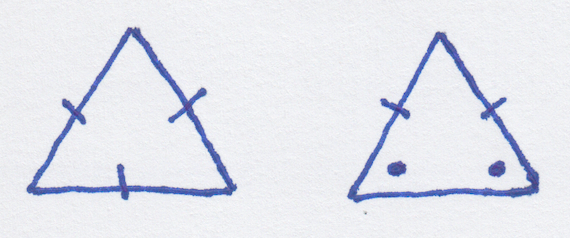
\includegraphics [scale=0.7] {G0.png} \end{center}

And then use it again.
\begin{center} 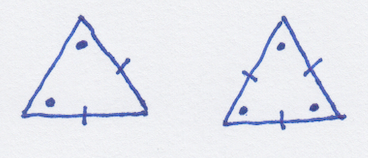
\includegraphics [scale=1.2] {G1.png} \end{center}

We see that an equilateral triangle has all three angles equal as well.  Thus each angle is $180 \div 3 = 60$.

Looking back at our proof of the isosceles triangle theorem, 
\begin{center} 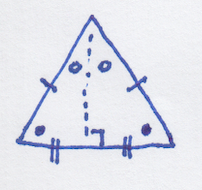
\includegraphics [scale=1.2] {G2.png} \end{center}

The angle at the top is bisected, so each half is $30$.  That matches the base of the altitude, which is a right angle.  We have two 30-60-90 right triangles and the two smaller angles in each of those small triangles add up to one right angle.  The base is also bisected.  

Let's look at some ratios of lengths.  It is most convenient to let one-half of the base have length $1$, so then the side is $2$.
\begin{center} 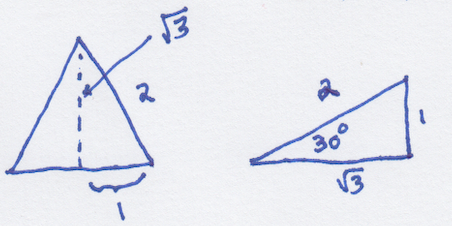
\includegraphics [scale=0.8] {G3.png} \end{center}
The third side comes from the Pythagorean theorem:
\[ 2^2 = 1^2 + h^2 \]
\[ h = \sqrt{3} \]

\subsection*{inscribed triangle}

We want to draw an equilateral triangle with each of its vertices in the same circle, called a circumcircle.  Start by drawing a diameter of the circle, vertically.

Anticipating the next result, to draw the base of the triangle, divide the radius from the center to the bottom of the circle in half ($PM = MT$), then draw a horizontal line $QS$ there.  Draw $QR$ and $SR$ to the apex at the top.
\begin{center} 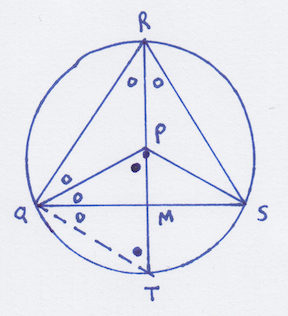
\includegraphics [scale=0.5] {G7.png} \end{center}

$QS$ is called a "chord" of the circle.  Since we've drawn it perpendicular to the radius $PT$, the resulting $\triangle PMQ \cong \triangle PMS$ by hypotenuse-leg in a right triangle.  The extension of the radius to $R$ forms a shared side for two triangles $\triangle RMQ$ and $\triangle RMS$.  Since $RM$ is shared and $QM = MS$, and the angles at $M$ are right angles, these two triangles are also congruent.

Therefore, the diameter bisects the angle at vertex $R$, each half marked with an open dot.  The angle $\angle RQP$ is equal by the isosceles triangle theorem.  $\angle RQP = \angle PQM$ for the same reason as the angle at $R$ is bisected, because $QP$ is a diameter of the circle drawn through the vertex at $Q$.

Lastly, the two angles $\angle RQP$ and $\angle PQM$ together form one whole angle of an equilateral triangle, which is two-thirds of a right angle, but $\angle RQT$ is a right angle, by Thales' theorem.  So $\angle MQT$ is equal to the others.

This construction also forms a smaller $\triangle PQT$.  We can use algebra to show that it is equilateral.  The right angle contains three of the dotted angles, so $\angle PQT$ contains two, and since $\triangle QPT$ contains two radii of the circle $\angle PQT = \angle QTP$.  We get the third angle from the triangle sum theorem.
\begin{center} 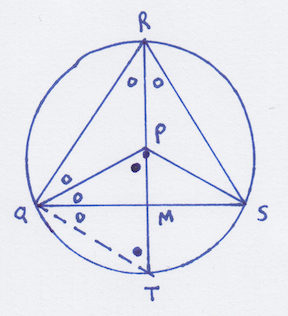
\includegraphics [scale=0.5] {G7.png} \end{center}

Another way to see that is to use the inscribed angle theorem and show that $\angle QTP = \angle QSR$, because they are both peripheral angles that cut off the same arc of the circle.

We wonder about the distance from the base of the triangle to the center, $PM$.  It's the same as the distance as $MT$, by construction.  So $MT$ is one-half the radius.

Hence the distance $RM$ is one whole radius plus a half.  So the distance from the base to the center at $P$ divided by the whole altitude is
\[ \frac{1/2}{3/2} = \frac{1}{3} \]

\begin{center} 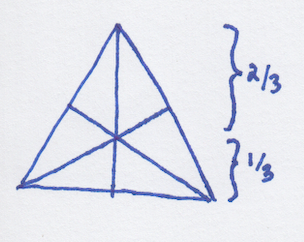
\includegraphics [scale=1.0] {G6.png} \end{center}

The place where lines like this meet has various names, depending on how the lines are chosen.  Since we're talking about altitudes of the triangle, the point is called the orthocenter.

Another way to calculate $MT$ is to use similar triangles.  That length is one-half the base of $\triangle QPT$, so it  is to its altitude ($1/2$ of $RS$, which is $1/2 \cdot 2 = 1$) as the ratio $1/\sqrt{3}$ in the large triangle.
\[ MT = \frac{1}{\sqrt{3}} \]

Hence the ratio of $MT$ to the altitude of the large triangle is
\[ \frac{1/\sqrt{3}}{\sqrt{3}} = \frac{1}{3}  \]

as we said.

\subsection*{hexagon}

A hexagon can be composed of six equilateral triangles.  One reason is that the whole central angle of 360 is divided into six equal parts, so each triangle has central angle of 60, but it is also isosceles, so the other angles are 60 as well..  

\begin{center} 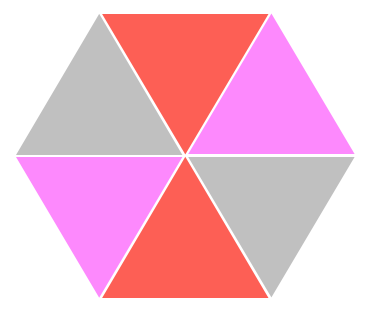
\includegraphics [scale=0.4] {hexagon.png} \end{center}

We notice that walking along the perimeter, at each turn we go 60 to the left, meaning that the inside angle is 120 or twice 60.

There is a famous theorem, usually proved by induction, that the sum of internal angles in any polygon is equal to 180 times the number of sides greater than 3, plus 180.  Here, that number is 3, giving 180(3) + 180 = 720.  

You can easily confirm that 6(180) = 720.  It's worth thinking about why that theorem makes sense.  Hint:  it has to do with the fact that a 4-sided figure can be cut into 2 triangles, a 5-sided figure into 3, and a 6-sided figure into 4.


\end{document}
